\documentclass[8pt,aspectratio=169]{beamer}
\usetheme{Madrid}
\usepackage{graphicx}
\usepackage{booktabs}
\usepackage{adjustbox}
\usepackage{multicol}
\usepackage{amsmath}
\usepackage{amssymb}
\usepackage{tikz}
\usetikzlibrary{arrows.meta,positioning,shapes.callouts,shapes.geometric,decorations.pathreplacing}
\usepackage{hyperref}
\usepackage{algorithm}
\usepackage{algorithmic}

% Color definitions
\definecolor{mlblue}{RGB}{0,102,204}
\definecolor{mlpurple}{RGB}{51,51,178}
\definecolor{mllavender}{RGB}{173,173,224}
\definecolor{mllavender2}{RGB}{193,193,232}
\definecolor{mllavender3}{RGB}{204,204,235}
\definecolor{mllavender4}{RGB}{214,214,239}
\definecolor{mlorange}{RGB}{255, 127, 14}
\definecolor{mlgreen}{RGB}{44, 160, 44}
\definecolor{mlred}{RGB}{214, 39, 40}
\definecolor{mlgray}{RGB}{127, 127, 127}

% Additional colors for template compatibility
\definecolor{lightgray}{RGB}{240, 240, 240}
\definecolor{midgray}{RGB}{180, 180, 180}

% Backward compatibility: uppercase color names
\colorlet{MLPurple}{mlpurple}
\colorlet{MLBlue}{mlblue}
\colorlet{MLOrange}{mlorange}
\colorlet{MLGreen}{mlgreen}
\colorlet{MLRed}{mlred}
\colorlet{MLLavender}{mllavender}
\colorlet{MLGray}{mlgray}

% Apply custom colors to Madrid theme
\setbeamercolor{palette primary}{bg=mllavender3,fg=mlpurple}
\setbeamercolor{palette secondary}{bg=mllavender2,fg=mlpurple}
\setbeamercolor{palette tertiary}{bg=mllavender,fg=white}
\setbeamercolor{palette quaternary}{bg=mlpurple,fg=white}

\setbeamercolor{structure}{fg=mlpurple}
\setbeamercolor{section in toc}{fg=mlpurple}
\setbeamercolor{subsection in toc}{fg=mlblue}
\setbeamercolor{title}{fg=mlpurple}
\setbeamercolor{frametitle}{fg=mlpurple,bg=mllavender3}
\setbeamercolor{block title}{bg=mllavender2,fg=mlpurple}
\setbeamercolor{block body}{bg=mllavender4,fg=black}

% Remove navigation symbols
\setbeamertemplate{navigation symbols}{}

% Clean itemize/enumerate
\setbeamertemplate{itemize items}[circle]
\setbeamertemplate{enumerate items}[default]

% Reduce margins for more content space
\setbeamersize{text margin left=5mm,text margin right=5mm}

% Custom course footer
\setbeamertemplate{footline}{
  \leavevmode%
  \hbox{%
    \begin{beamercolorbox}[wd=.333333\paperwidth,ht=2.25ex,dp=1ex,center]{author in head/foot}%
      \usebeamerfont{author in head/foot}Methods and Algorithms
    \end{beamercolorbox}%
    \begin{beamercolorbox}[wd=.333333\paperwidth,ht=2.25ex,dp=1ex,center]{title in head/foot}%
      \usebeamerfont{title in head/foot}MSc Data Science
    \end{beamercolorbox}%
    \begin{beamercolorbox}[wd=.333333\paperwidth,ht=2.25ex,dp=1ex,right]{date in head/foot}%
      \usebeamerfont{date in head/foot}\insertframenumber{} / \inserttotalframenumber\hspace*{2ex}
    \end{beamercolorbox}}%
  \vskip0pt%
}

% Command for bottom annotation (Madrid-style)
\newcommand{\bottomnote}[1]{%
\vfill
\vspace{-2mm}
\textcolor{mllavender2}{\rule{\textwidth}{0.4pt}}
\vspace{1mm}
\footnotesize
\textbf{#1}
}

% Custom commands for course compatibility
\newcommand{\highlight}[1]{\textcolor{mlorange}{\textbf{#1}}}
\newcommand{\mathbold}[1]{\boldsymbol{#1}}

\title[L04: DT \& RF Visuals]{Decision Trees \& Random Forests: The Essential Visuals}
\subtitle{20 Key Charts Every Data Scientist Should Know}
\author{Methods and Algorithms}
\date{Spring 2026}

\begin{document}

% ============================================================
% FRONT MATTER
% ============================================================

% SLIDE 1: Title Page
\begin{frame}
\titlepage
\end{frame}

% SLIDE 2: Opening XKCD
\begin{frame}[t]{The Machine Learning Pipeline}
\vspace{0.5em}
\begin{center}

\includegraphics[height=0.55\textheight]{images/1838_machine_learning.png}
\end{center}
\bottomnote{XKCD \#1838 by Randall Munroe (CC BY-NC 2.5)}
\end{frame}

% SLIDE 3: Learning Objectives
\begin{frame}[t]{Learning Objectives}
\vspace{1em}
After this lecture, you will be able to:
\begin{itemize}
  \item \textbf{Visualize} how decision trees partition feature space
  \item \textbf{Understand} the bias--variance tradeoff in tree models
  \item \textbf{See} how random forests improve over single trees
  \item \textbf{Interpret} RF models using modern diagnostic tools
\end{itemize}
\bottomnote{We cover 20 essential visualizations spanning foundations, ensemble mechanics, and model interpretation}
\end{frame}

% SLIDE 4: Table of Contents
\begin{frame}{Outline}
  \tableofcontents
\bottomnote{Three parts: Decision Tree Foundations, Random Forest Power, Interpretation and Evaluation}
\end{frame}

% ============================================================
% PART 1: DECISION TREE FOUNDATIONS (7 charts)
% ============================================================
\section{Decision Tree Foundations}

% SLIDE 5: C1 --- Decision Boundary
\begin{frame}[t]{How Does a Decision Tree Classify?}
\begin{center}

\includegraphics[width=0.65\textwidth]{10_dt_decision_boundary/chart.pdf}
\end{center}
\bottomnote{Decision trees create axis-aligned rectangular partitions of the feature space}
\end{frame}

% SLIDE 6: C4 --- Gini & Entropy
\begin{frame}[t]{Impurity Measures: Gini vs Entropy}
\begin{center}

\includegraphics[width=0.65\textwidth]{11_gini_vs_entropy/chart.pdf}
\end{center}
\bottomnote{Both measures reach maximum at $p=0.5$ (maximum uncertainty) and minimum at $p=0$ or $p=1$ (pure nodes)}
\end{frame}

% SLIDE 7: C5 --- Tree Structure (NEW)
\begin{frame}[t]{Inside the Tree: Nodes, Splits, and Leaves}
\begin{center}

\includegraphics[width=0.65\textwidth]{top10_05_tree_structure/chart.pdf}
\end{center}
\bottomnote{Each node shows the split rule, impurity measure, sample count, and class distribution}
\end{frame}

% SLIDE 8: C3 --- DT Regression Step
\begin{frame}[t]{Decision Tree Regression: Piecewise Approximation}
\begin{center}

\includegraphics[width=0.65\textwidth]{16_regression_tree_mse/chart.pdf}
\end{center}
\bottomnote{Decision trees approximate continuous functions with piecewise-constant (step) predictions}
\end{frame}

% SLIDE 9: C2 --- Bias-Variance Tradeoff
\begin{frame}[t]{The Core Tradeoff: Tree Depth vs Error}
\begin{center}

\includegraphics[width=0.65\textwidth]{17_bias_variance_depth/chart.pdf}
\end{center}
\bottomnote{Shallow trees underfit (high bias); deep trees overfit (high variance). The optimal depth minimizes test error.}
\end{frame}

% SLIDE 10: A2 --- Validation Curve (NEW)
\begin{frame}[t]{Validation Curve: Finding Optimal Depth}
\begin{center}

\includegraphics[width=0.65\textwidth]{top10_12_validation_curve/chart.pdf}
\end{center}
\bottomnote{Cross-validated train and test scores reveal the sweet spot between underfitting and overfitting}
\end{frame}

% SLIDE 11: A9 --- Leaf Purity (NEW)
\begin{frame}[t]{Leaf Node Purity: Shallow vs Deep Trees}
\begin{center}

\includegraphics[width=0.65\textwidth]{top10_19_leaf_purity/chart.pdf}
\end{center}
\bottomnote{Deeper trees produce purer leaves but risk memorizing noise in the training data}
\end{frame}

% ============================================================
% TRANSITION
% ============================================================

% SLIDE 12: Transition
\begin{frame}[t]{The Problem: Single Trees Are Unstable}
\vspace{1.5em}
\begin{itemize}
  \item Small changes in data $\rightarrow$ very different tree structures
  \item Deep trees memorize noise (\highlight{overfitting})
  \item \textbf{Solution:} Combine many diverse trees $\rightarrow$ \highlight{Random Forest}
\end{itemize}
\bottomnote{The instability of individual trees is a feature, not a bug---it creates the diversity that makes ensembles work}
\end{frame}

% ============================================================
% PART 2: RANDOM FOREST POWER (6 charts)
% ============================================================
\section{Random Forest Power}

% SLIDE 13: C8 --- DT vs RF Boundary (NEW)
\begin{frame}[t]{The Ensemble Effect: Smooth Boundaries}
\begin{center}

\includegraphics[width=0.65\textwidth]{top10_08_dt_vs_rf_boundary/chart.pdf}
\end{center}
\bottomnote{Averaging 200 trees smooths out the jagged decision boundary of a single tree}
\end{frame}

% SLIDE 14: C7 --- OOB Convergence
\begin{frame}[t]{How Many Trees Are Enough?}
\begin{center}

\includegraphics[width=0.65\textwidth]{27_rf_ntrees_convergence/chart.pdf}
\end{center}
\bottomnote{OOB error provides free cross-validation; error plateaus after 100--200 trees}
\end{frame}

% SLIDE 15: C9 --- max\_features Effect
\begin{frame}[t]{The Key Hyperparameter: max\_features}
\begin{center}

\includegraphics[width=0.65\textwidth]{18_rf_hyperparameter_maxfeatures/chart.pdf}
\end{center}
\bottomnote{Reducing features per split decorrelates trees, improving ensemble diversity at the cost of individual tree accuracy}
\end{frame}

% SLIDE 16: A1 --- Learning Curve (NEW)
\begin{frame}[t]{Learning Curves: Decision Tree vs Random Forest}
\begin{center}

\includegraphics[width=0.65\textwidth]{top10_11_learning_curve/chart.pdf}
\end{center}
\bottomnote{Random forests generalize better than single trees, especially with limited training data}
\end{frame}

% SLIDE 17: A6 --- Probability Heatmap (NEW)
\begin{frame}[t]{Prediction Probability Landscape}
\begin{center}

\includegraphics[width=0.65\textwidth]{top10_16_probability_heatmap/chart.pdf}
\end{center}
\bottomnote{Unlike hard classifications, predict\_proba reveals model confidence across the feature space}
\end{frame}

% SLIDE 18: A8 --- Ensemble Diversity (NEW)
\begin{frame}[t]{Why Diversity Matters: Tree Disagreement}
\begin{center}

\includegraphics[width=0.55\textwidth]{top10_18_ensemble_diversity/chart.pdf}
\end{center}
\bottomnote{Feature randomization ensures trees disagree on individual predictions while agreeing on the overall}
\end{frame}

% ============================================================
% PART 3: INTERPRETATION & EVALUATION (7 charts)
% ============================================================
\section{Interpretation and Evaluation}

% SLIDE 19: C6 --- Feature Importance
\begin{frame}[t]{Which Features Matter Most?}
\begin{center}

\includegraphics[width=0.65\textwidth]{02_feature_importance/chart.pdf}
\end{center}
\bottomnote{Mean Decrease in Impurity (MDI) ranks features by how much they reduce node impurity across all trees}
\end{frame}

% SLIDE 20: C10 --- Partial Dependence (NEW)
\begin{frame}[t]{Partial Dependence: Feature Effects}
\begin{center}

\includegraphics[width=0.65\textwidth]{top10_10_partial_dependence/chart.pdf}
\end{center}
\bottomnote{PDPs show the marginal effect of a feature on predictions, averaging out all other features}
\end{frame}

% SLIDE 21: A7 --- 2D PDP Contour (NEW)
\begin{frame}[t]{Feature Interaction: 2D Partial Dependence}
\begin{center}

\includegraphics[width=0.65\textwidth]{top10_17_2d_pdp_contour/chart.pdf}
\end{center}
\bottomnote{2D PDPs reveal interaction effects between two features that 1D plots cannot capture}
\end{frame}

% SLIDE 22: A3 --- ROC Comparison (NEW)
\begin{frame}[t]{ROC Curves: Single Tree vs Forest}
\begin{center}

\includegraphics[width=0.65\textwidth]{top10_13_roc_comparison/chart.pdf}
\end{center}
\bottomnote{Random forests typically achieve higher AUC than single trees due to lower variance in probability estimates}
\end{frame}

% SLIDE 23: A4 --- Confusion Matrix (NEW)
\begin{frame}[t]{Confusion Matrix: Reading the Results}
\begin{center}

\includegraphics[width=0.65\textwidth]{top10_14_confusion_matrix/chart.pdf}
\end{center}
\bottomnote{In fraud detection, minimizing false negatives (missed fraud) is often more important than minimizing false positives}
\end{frame}

% SLIDE 24: A5 --- Calibration Curve (NEW)
\begin{frame}[t]{Are the Probabilities Reliable?}
\begin{center}

\includegraphics[width=0.65\textwidth]{top10_15_calibration_curve/chart.pdf}
\end{center}
\bottomnote{Well-calibrated models have predicted probabilities that match observed frequencies}
\end{frame}

% SLIDE 25: A10 --- Proximity Matrix (NEW)
\begin{frame}[t]{Random Forest Proximity: Which Samples Are Similar?}
\begin{center}

\includegraphics[width=0.55\textwidth]{top10_20_proximity_matrix/chart.pdf}
\end{center}
\bottomnote{Samples landing in the same leaves are considered similar by the forest}
\end{frame}

% ============================================================
% CLOSING
% ============================================================
\section{Summary}

% SLIDE 26: Summary Checklist
\begin{frame}[t]{20 Charts You Should Know}
\vspace{0.3em}
\begin{columns}[T]
\begin{column}{0.48\textwidth}
\footnotesize
\begin{enumerate}
  \item Decision Boundary
  \item Gini \& Entropy
  \item Tree Structure
  \item Regression Fit
  \item Bias--Variance
  \item Validation Curve
  \item Leaf Purity
  \item DT vs RF Boundary
  \item OOB Convergence
  \item max\_features
\end{enumerate}
\end{column}
\begin{column}{0.48\textwidth}
\footnotesize
\begin{enumerate}
  \setcounter{enumi}{10}
  \item Learning Curves
  \item Probability Landscape
  \item Ensemble Diversity
  \item Feature Importance
  \item Partial Dependence
  \item 2D PDP Interaction
  \item ROC Comparison
  \item Confusion Matrix
  \item Calibration Curve
  \item Proximity Matrix
\end{enumerate}
\end{column}
\end{columns}
\bottomnote{These 20 visualizations cover the foundations, mechanics, and interpretation of tree-based models}
\end{frame}

% SLIDE 27: Closing XKCD
\begin{frame}[t]{The Wisdom of the Crowd}
\vspace{0.5em}
\begin{center}
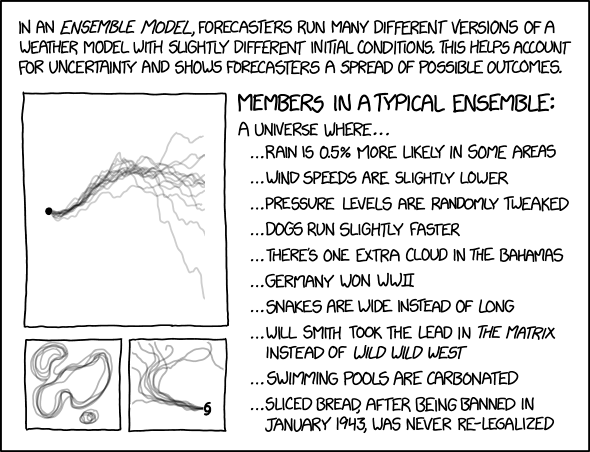
\includegraphics[height=0.55\textheight]{images/1885_ensemble_model.png}
\end{center}
\bottomnote{XKCD \#1885 by Randall Munroe (CC BY-NC 2.5)}
\end{frame}

\end{document}
